\documentclass[letterpaper]{article}
\title{CS589 Machine Learning, Fall 2020 \\ \ \\ \large{Assignment 1: Discriminative Models - Regression}}

\date{Due: September 11th, 07:00 PM}

\usepackage[margin=1in]{geometry}
% \usepackage{hyperref}
\usepackage[colorlinks]{hyperref}
\usepackage{capt-of}
\usepackage{amssymb}
\usepackage{amsmath}
\usepackage{url}
\usepackage{graphicx}
\usepackage{color}
\usepackage{bbm}
\usepackage{float}
\def\argmin{\mathop{\text{arg\,min}}}
\def\argmax{\mathop{\text{arg\,max}}}
\newcommand{\cov}{\mathrm{cov}}
\newcommand{\E}{\mathbb{E}}

%\newcommand{\sol}{1}

\newcommand{\Solution}[1]{\paragraph{\bf $\bigstar $ SOLUTION:} { \sf
    #1} \bigskip}
\begin{document}

{\centering
  \rule{6.3in}{2pt}
  \vspace{1em}
  {\Large
    CS589 Machine Learning - Fall 2020 \\
    Homework 1: Classification \\
  }
  \vspace{1em}
  Due: September 11th, 07:00 PM \\
  \vspace{0.1em}
  \rule{6.3in}{1.5pt}
}
\vspace{1pc}

%\maketitle

\paragraph*{Getting Started:} You should complete the assignment using your own installation of Python 3.6. Download the assignment archive from Moodle and unzip the file. This will create the directory structure as shown below. You will write your code under the Submission/Code directory. Make sure to put the deliverables (explained below) into the respective directories.

\begin{verbatim}
HW01
--- Data
    |-- Credit Card Transaction
--- Submission
    |--Code
    |--Predictions
\end{verbatim}

If you are stuck on a question consider attending the office hours for that question.

\paragraph*{Data Sets:} It is important that credit card companies are able to recognize fraudulent credit card transactions so that customers are not charged for items that they did not purchase. In this assignment, you will experiment with different classifiers on the binary classification problem of anomaly detection in credit card transactions. The dataset described below contains transactions that occurred in a two day period. Due to confidentiality issues, the background information about the features will not be described. You only know that the first attribute describes the dollar amount in the transaction and the class output is either 0 for normal or 1 for fraud. \vspace{12pt}

\begin{table}[h!]
\center
\begin{tabular}{|l|c|c|c|c|}\hline
Dataset & Training Cases & Test Cases & Dimensionality & Number of Classes\\\hline
Credit Card Transaction & 200000 & 50000 & 29 & 2\\\hline
\end{tabular}
\end{table}

\paragraph*{Deliverables:} This assignment has two types of deliverables: a report and the code files. 
\begin{itemize}
\item \textbf{Report: } The solution report will give your answers to the homework questions (listed below). The maximum length of the report is 5 pages in 11 point font, including all figures and tables. You can use any software to create your report, but your report must be submitted in PDF format. 

\item \textbf{Code: } The second deliverable is the code that you wrote to answer the questions, which will involve training classifiers and making predictions on held-out test data. Your code must be Python 3.6 (no iPython notebooks, other formats or code from other versions). You may create any additional source files to perform data analysis. However, you should aim to write your code so that it is possible to re-produce all of your experimental results exactly by running \textit{python run\_me.py} file from the Submissions/Code directory. Remember to comment your code. Points will be deducted from your assignment grade if your code is difficult to reproduce!

\end{itemize}

\paragraph*{Submitting Solutions:} When you complete the assignment, place your final code in \textbf{Submission/Code}, and the prediction files for your single best-performing submission in \textbf{Submission/Predictions/best.csv}. Finally, create a zip file called \textbf{Submission.zip} from your \textbf{Submission} directory only (do not include `Data' directory). Only .zip files will be accepted for grading code (not .tar, .rar, .gz, etc.). You will upload your .zip file of code and your pdf report to Gradescope for grading. Further instructions for using Gradescope will be provided on Piazza and discussed in class.

\paragraph*{Academic Honesty Statement:} Copying solutions from external sources (books, web pages, etc.) or other students is considered cheating. Sharing your solutions with other students is  considered cheating. Posting your code to public repositories like GitHub is also considered cheating. Any detected cheating will result in a grade of 0 on the assignment for all students involved, and potentially a grade of F in the course.\\


\section{Probability and Estimation [30 points]}

\begin{enumerate}

   \item {[10 points]} Let's take a look at a classical problem in document classification. Each document is associated with a pair $(\vec{w}, y)$, where $\vec{w}$ is a feature vector of word counts of the document and y is the label for whether the document is useful (y=1 if yes, y=0 if no). The vocabulary is of size 3, so each component of the feature vector $(w_1, w_2, w_3)$ refers to a discrete variable that corresponds to the word count of the word type in the document, some feature vectors $\vec{w}$ look like (0, 1, 5), (1, 2, 1), etc. 
  
Consider a naive Bayes model with the following conditional probability table
\begin{table}[!htbp]
\centering
\begin{tabular}{|c|c|c|c|}
\hline
word type         & 1   & 2   & 3    \\
\hline
$P(w \mid y = 1)$ & 0.2 & 0.3 & 0.5 \\
\hline
$P(w \mid y = 0)$ & 0.4 & 0.5 & 0.1  \\
\hline
\end{tabular}
\end{table}

and the following prior probabilities over classes:
\begin{table}[!htbp]
\centering
\begin{tabular}{|c|c|}
\hline
$P(y=1)$ & 0.3   \\
\hline
$P(y=0)$ & 0.7  \\
\hline
\end{tabular}
\end{table}

Now, we have a document with counts $\vec{x} = (0, 1, 1)$. Which class has higher posterior probability? What is the posterior probability that the document is relevant/useful? What is the naive assumption in this problem?
   
 
  \item {[10 points]} Assume we have $N$ samples, $x_{1},...,x_{N}$ independently drawn from a normal distribution with known variance $\sigma^{2}$ and unknown mean $\mu$. Derive the maximum likelihood estimator (MLE) for the mean $\mu$.

 
  \item {[10 points]} Mathematically show how the MAP estimation equals the MLE estimation plus an additional term, $\log P(\theta)$. Then, explain whether there are situations under which the MLE and MAP estimators turn out to be identical.
  
  
\end{enumerate}


\section{K Nearest Neighbors [25 points]}

KNN is a data driven, instance-based learning algorithm. In classification, it assigns a new object to the class most common among its k nearest neighbors present from the training dataset. 

\begin{enumerate}

\item {[10 points]} Sketch a rough 1-nearest neighbor decision boundary for this dataset in the figure. In the example, why might a too large or too small value for $k$ be bad? Explain the bias-variance tradeoff and how it pertains to the scenario in KNN. What value of $k$ minimizes leave-one-out cross-validation error for this dataset, and what is the resulting error? (See \href{https://en.wikipedia.org/wiki/Cross-validation\_(statistics)\#Leave-one-out\_cross-validation}{leave-one-out cross-validation wiki page} if not familiar with leave-one-out cross-validation)

\begin{center}
\includegraphics[width=5cm,height=5cm,keepaspectratio]{knn.pdf} \\*
\end{center}



\item {[10 points]} For the Credit Card Transaction Dataset, train 5 different nearest neighbors regressors using the following number of neighbors: 3, 5, 10, 20, and 25. Report the out of sample F1 score using your own implementation of 5-fold cross-validation. F1 score is defined as the harmonic mean of precision and recall.
\[ precision = \frac{\# \, true \, positives}{\# \, true \, positives + \# \, false \, positives} \]
\[ recall = \frac{\# \, true \, positives}{\# \, true \, positives + \# \, false \, negatives} \]
\[ F_{1} score = 2 * \frac{precision * recall}{precision + recall} \]

\item {[5 points]} Why does it make more sense to use F1 score as the evaluation metric over classification accuracy in our problem domain?

\end{enumerate}


\section{Decision Trees [25 points]}

The decision tree model predicts the value of a target variable by learning simple decision rules inferred from the data features. It is easy to interpret and have powerful performance when combined with ensemble methods, which we'll cover later on in the course.

\begin{enumerate}
  \item {[10 points]} What is the criteria used to select a variable for a node when training a decision tree? Is it optimal? If yes, explain why it is optimal. If no, explain why is the optimal ordering not used.
  

  \item {[10 points]} For the Credit Card Transaction Dataset, train 5 different decision trees with the following maximum depths: 3, 6, 9, 12, and 15. Report the out of sample F1 score using your own implementation of 5-fold cross-validation. In addition, measure the time (in milliseconds) that it takes to perform cross-validation with each model and report the results using a graph. 
  
  \item {[5 points]} Now, try optimizing your decision tree model by running either a randomized search or grid search on the other hyperparameters that you see fit. Did the model performance improve? Report what you did, the best set of hyper-parameters you found, and the out of sample five-fold cross-validation you achieved. 

\end{enumerate}


\section{Model Selection \& Hyperparameter Tuning [10 points]}

 \begin{enumerate}

\item {[5 points]} Consider the machine learning algorithms taught in class: KNN, decision trees, and logistic regressions. Which of these are considered high bias, and which of these are low bias? Explain. 

 
\item {[5 points]} To perform $k$-fold cross-validation, you split a dataset of $N$ samples into $k$ subsets of size $N/k$. Suppose that training a model on a dataset with $M$ samples takes $M$ units of time, and the time that it takes to evaluate the model is negligible. What is the time complexity in big-O notation of performing cross-validation on such a model? What happens if $k = 5$? What happens if $k = N$ (aka ``leave one out'' cross validation)? How does the choice of $k$ trade off computational complexity against the quality of the estimate?

 
 
\end{enumerate}


\section{Train Your Best Model [10 points]}

\begin{enumerate}
\item {[10 points]} 
Now, for the Credit Card Transaction Dataset, you may use any model you like that has been taught in class or covered in the homework. Build you model, train the model using the training set however you want, then generate predictions of the test set, and save the outputs into the \textbf{Submission/Predictions} folder. Finally, describe your model selection, why you selected the model, how you tuned/choosed the hyperparameters (if applicable), and report both the metrics on the average validation from 5-fold cross validation and the full training set with your best performing model. The metrics should be reported in a table like this:\\
\begin{table}[h!]
\center
\begin{tabular}{|l|c|c|c|c|}\hline
Metric              & Precision & Recall & F1 Score & AUC \\\hline
Avg. Validation Set &           &        &          &     \\\hline
Full Training Set   &           &        &          &     \\\hline
\end{tabular}
\end{table}

\textbf{Hints:}
\begin{itemize}
    \item Split the training set however you want to find your best model.
    \item Run a 5-fold cross validation with your best model, and report the average results of the 5 validation sets.
    \item Run the best performing model on the full training set, and report the result of that.
    \item Run the best performing model on the test set, and save the predictions.
\end{itemize}

For this question \textbf{only}, usage of \textbf{scikit-learn} is allowed to search for the best performing model. For more information 
on the AUC (area under curve) metric, please refer to online resources such as https://towardsdatascience.com/understanding-auc-roc-curve-68b2303cc9c5. 
\begin{center}
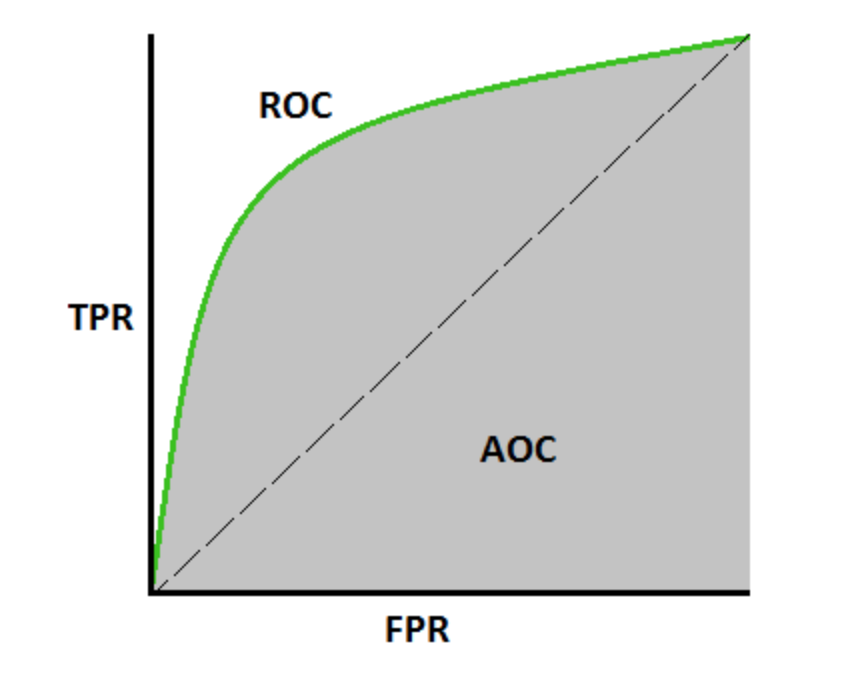
\includegraphics[width=5cm,height=5cm,keepaspectratio]{auc.png} \\*
\end{center}
\end{enumerate}



\end{document}
